\section{Performances}
\subsection{\textit{3blocsSimple} example}
With the following configuration:
\begin{itemize}
\item \textbf{Number of processes}: 4
\item \textbf{$\sigma$}: 0.51
\item \textbf{bandwidth}: 1.5
\end{itemize}
We get the same results for Spectral clustering and Mean shift(see Figure \ref{3blocsSimple}). The computation times are also similar:
\begin{itemize}
\item \textbf{Spectral Clustering}: 0.105 s
\item \textbf{Mean Shift}: 0.120 s
\end{itemize}
\begin{figure}[h!]
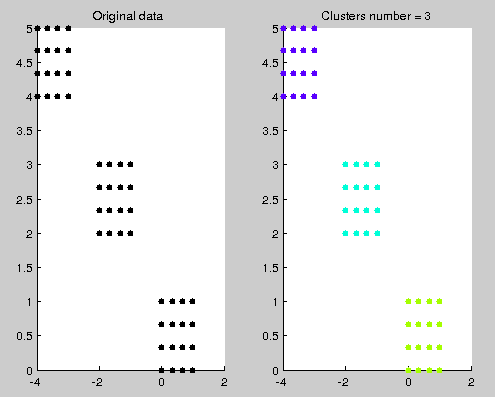
\includegraphics[width=0.5\textwidth, height=5.5cm]{Image/3blocsSimple.png}\centering
\caption{\textit{3blocsSimple} result\label{3blocsSimple}}
\end{figure}

\subsection{\textit{croix16} example}
With the following configuration:
\begin{itemize}
\item \textbf{Number of processes}: 1
\item \textbf{$\sigma$}: 0.51
\item \textbf{bandwidth}: 1.5
\end{itemize}
We get the same results for Spectral clustering and Mean shift(see Figure \ref{croix16}). However we obtained a faster execution for Mean Shift:
\begin{itemize}
\item \textbf{Spectral Clustering}: 18.32 s
\item \textbf{Mean Shift}: 4.106E-2 s
\end{itemize}
\begin{figure}[h!]
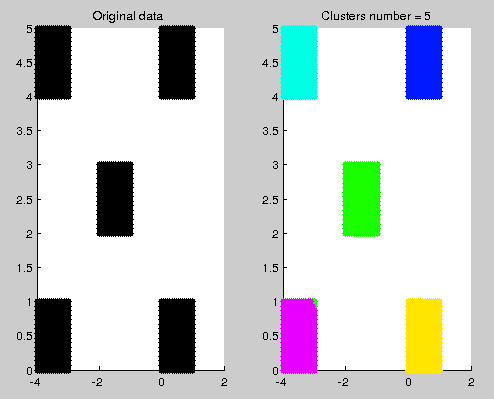
\includegraphics[width=0.5\textwidth]{Image/croix16.png}\centering
\caption{\textit{croix16} result\label{croix16}}
\end{figure}
